%% This is an example first chapter.  You should put chapter/appendix that you
%% write into a separate file, and add a line \include{yourfilename} to
%% main.tex, where `yourfilename.tex' is the name of the chapter/appendix file.
%% You can process specific files by typing their names in at the 
%% \files=
%% prompt when you run the file main.tex through LaTeX.

fix the abstract to include UPC (currently only FIB is shown)
\cite{Darwin} \cite{Crockford} \cite{Stefanov} \cite{AngularJSGuide} \cite{Fowler}


\chapter{Introduction}
% possible quotations: welcome humans. goodwill. and we have a plan.
stuff that should be somewhere: DSL, TDD, .deb, linux and tools, debugging,etc opensourcing. DRY and DRA (do not repeat angularjs docs), xml (our lang) and how we use it (themes, inheritance, composition, urls), restful/services to fetch API data
why angularjs instead of, say, a lemon.

\section{PAL Robotics}
Pal Robotics is a company based in Barcelona dedicated to R\&D of humanoid robots and robotic components. 
An international team of mostly mechanical, electronics and software engineers pushes forward the research on different fields, like speech recognition and generation, computer vision, walking, grasping, machine learning and navigation amongst others.
The company has developed 5 humanoid robots in 2013: Reem-A, Reem-B, Reem H1, H2 and H3, and Reem-C (still in the labs).
This project targets Reem H2 and H3.

\subsection{Reem H2 and H3}
Reem H2 and H3 are service robots featuring a screen on their torso.
They have an autonomous navigation system, speech recognition and synthetiser, they can find their way in different settings and help or entertain people in a friendly way.
They can be used in public places such as hotels, malls, airports or museums.

% mini page here.
%  rh2pic rh3pic
%  rh2tab rh3tab

\begin{table}[ht]
    \centering
    \caption{Reem H2}
    \label{tab:rh2}
    \begin{tabularx}{\linewidth}{| X | X |}
    \hline
    Weight & 90 Kg \\ \hline
    Height & 1.70 m \\ \hline
    Battery life & 8 h \\ \hline
    Degrees of freedom & 22 \\ \hline
    Payload & 30 Kg (mobile base), 3 Kg/arm \\ \hline
    Speed & 4 Km/h \\ \hline
    Computer & Core 2 Duo + Atom \\ \hline
    Sensors & Microphone, stereo-camera, laser, ultrasounds, accelerometers and gyroscopes \\
    \hline
    \end{tabularx}
\end{table}


\section{The Current System}
The Reem series have big potential in human robot interaction. 
Besides speech or joystick manual control, humans can use a touch screen to command the robot or obtain information.
Reem can display multimedia contents like corporate videos, information about the client, capabilities of the robot, language settings, etc.

\begin{figure}[htb]
    \label{fig:intro-system-overview}
    \centering
    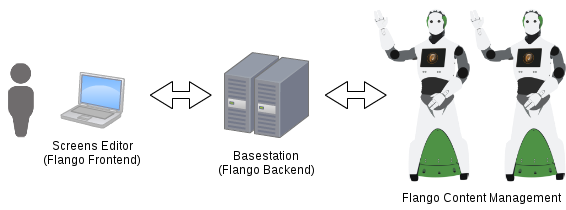
\includegraphics[width=\textwidth]{figures/intro-system-overview}
    \caption{Overview of the system}
\end{figure}

The Basestation is an application server that hosts Flango, an \ac{RIA} to manage contents and robots made with Django, a widely used framework for Python. 
Clients can create application contents with the Screens Editor, a tool built with Adobe Flex (c), in Flango.
When application contents are ready, clients can associate $1$ application with $n$ robots to display it in the touch screen.
The components of a contents application (screens and entities) have an \ac{XML} representation, an approach similar to popular projects (e.g. Android, NetBeans) and even, in an abstract way, all \acp{RIA} made with \ac{HTML}.

A contents application is essentially a set of screens, navigation, multimedia contents that users can manage with the media library, and entities. 
The last are domain objects that can be instantiated and represented in a view. 
This way a client can show information about the company, include buttons to provide an easy way to give commands to the robot (e.g. "follow me", "meet people"), display videos and picture galleries, etc.
All of these components are localisable. 
They can be resized, repositioned, repainted... depending on the current language.
This allows for more human-robot interaction and enriches the experience. 
Using other tools, clients can also associate sentences to screens and the speech synthesiser reads them aloud.

SCREENSHOT HERE

Reem robots have a built-in software to render the content applications that receive from Basestation. 
It is also made with Adobe Flex (c).
The main concern of this software is transforming \ac{XML} files into a \ac{UI}. 
This software has no \ac{GUI} or direct interaction with a person.

DIAGRAM HERE (screenshots?): XML --> software --> view

This thesis documents the project to re-engineer the built-in software in the robot to use modern web technologies.

\section{The New System}
The \ac{WWW} was born as a document viewing platform and has evolved gradually into an application platform. 
First the web consisted of truly pages that contained structured text and some images. 
Navigation was done using simple links between pages. 
In a second phase, web sites became interactive: 
it was the time of animated graphics, browser plug-ins and JavaScript. 
More recently web sites have adopted features from traditional desktop software in \acp{RIA}. \cite{Anttonen:2011}.

For a decade, the Adobe Flash Player plug-in has provided a platform to enable rich and interactive content in browsers.
However, Adobe has made the updates exclusive to the Google Chrome browser \cite{FlashRoadmap}. 
The browser in the robot application, QtWebBrowser (FIXME! it might be Chrome, in the end), uses this plug-in but will not receive updates from Adobe and PAL Robotics systems need to adapt to this new setting. 

The solution is moving to modern web technologies.
Any other technology could be used but the web allows the product to be easily portable, very extensible and open to many developers.
There are a number of options. \ac{HTML5} is perhaps the best known forthcoming standard in the Web and is typically combined with JavaScript and \ac{CSS3}. 
It has become such a popular combination that major browser vendors already provide an extensive support in a wide range of products.
A big number of frameworks with JavaScript have appeared not only client-side (e.g. BackBone, jQuery, Ext JS, Google Web Toolkit, YUI...), but even server-side (e.g. NodeJS).

The project documented in this thesis is using Google AngularJS, an \ac{MVC} framework that lets developers teach the browser new syntax. 
Thus, the syntax of the \ac{XML} files coming from the Screens Editor can be interpreted natively in a browser. 
This has some advantages over Flash \cite{Jobs:ThoughtsOnFlash}:
\begin{itemize}
    \item No use of third-party plug-ins
    \item Openness
    \item Reliability, security and performance
    \item Keeps power consumption lower (e.g. using the GPU to decode video or apply transformations and smooth transitions to elements on the screen)
    \item Touch-enabled: the new screen of Reem H3 is multi-touch. To enable gestures, heavy rewriting of the current Flash application is required.
\end{itemize}

\section{Context of the work}
TODO FIXME
The work context diagram identifies the boundaries of the work that you need to investigate to be able to build the product. Note that it includes more than the intended product. Unless we understand the work that the product will support, we have little chance of building a product that will fit cleanly into its environment.

The adjacent systems on the context diagram (e.g., Weather Forecasting Service) indicate other subject matter domains (systems, people, and organizations) that need to be understood. The interfaces between the adjacent systems and the work context indicate why we are interested in the adjacent system. In the case of Weather Forecasting Service, we can say that we are interested in the details of when, how, where, who, what, and why it produces the District Weather Forecasts information.

\section{Goals}
TODO: This section should probably be expanded

This thesis is part of the specialisation of Software Engineering and Information Systems. 
The goal is to develop an original high quality and fully functional software. 
More specifically, the author has to gather the requirements from an existing system, plan in terms of scope, time and cost, make the system specifications, design and implement it using modern web technologies, use quality assurance tools and deploy it successfully in a Reem H3 robot.

Regarding the project, the goals are:
\begin{itemize}
\item Reengineer the current system with web technologies
\item Develop a testing strategy to make it robust
\item Make it compatible with non-reengineered parts of the system
\end{itemize}

\section{Organisation of this document}
This document describes the system developed at PAL Robotics to render the screens created with the Screens Editor on the Reem H2 and H3 series.
It does not cover other software on the robots or in Basestation.

% TODO check the easy to read phrase
This project has been developed iteratively using a \ac{TDD} methodology. 
This document presents the system in a chronological manner as if it had followed classical software life cycle in its development, hoping to offer an easier reading:
It first analyses the state of the art and includes some background knowledge required to understand the decisions taken during the development, then the planning and the requirements, the specification of the system, the internal design (with special attention on the framework and the specific technology of both the hardware and the software), some examples of the implementation and the testing strategy.
Readers will find an overview section at the beginning of each chapter to put them in context.

\subsection{Conventions}
no conventions so far. thank you \LaTeX
